\documentclass[../Head/Main.tex]{subfiles}
\begin{document}
\section{Segmentation of Images} \label{sec:seg}
The code described in this section is found in the file \url{src/ex2.py}.\\
Four methods of segmentation are considered for distinguishing the orange pumpkins from the green background:
\begin{itemize}
\item Segmentation based on a range of RGB values
\item Segmentation based on a range of CieLAB values
\item Segmentation by histogram backprojection
\item Segmentation by a maximum euclidean distance from the mean RGB value
\end{itemize}

\subsection{Segmentation by Range of RGB Color Values}
The simplest method for segmentation to be applied is by only including pixels that are within some predefined color range. The range must be defined so as to include as much as possible of the pumpkin color range and exclude as much as possible of the color range in the remainder of the image.\\
Defining the allowed range for the different color channels was approached by examining the results of the color analysis described in section \ref{sec:colorAnalysis}. By looking at the histograms figure \ref{fig:histRgb} a proper lower boundary for all three RGB color channels would be the mean value minus one standard deviation and the upper boundary could be set to the mean value plus two standard deviations. In this way, the colors of the pumpkins would be approximately seperated from the remaining colors without too much overlap. Part of the segmented image drawed back on the original image can be seen in figure \ref{fig:bgrSeg}.

\begin{figure}[H]
\centering
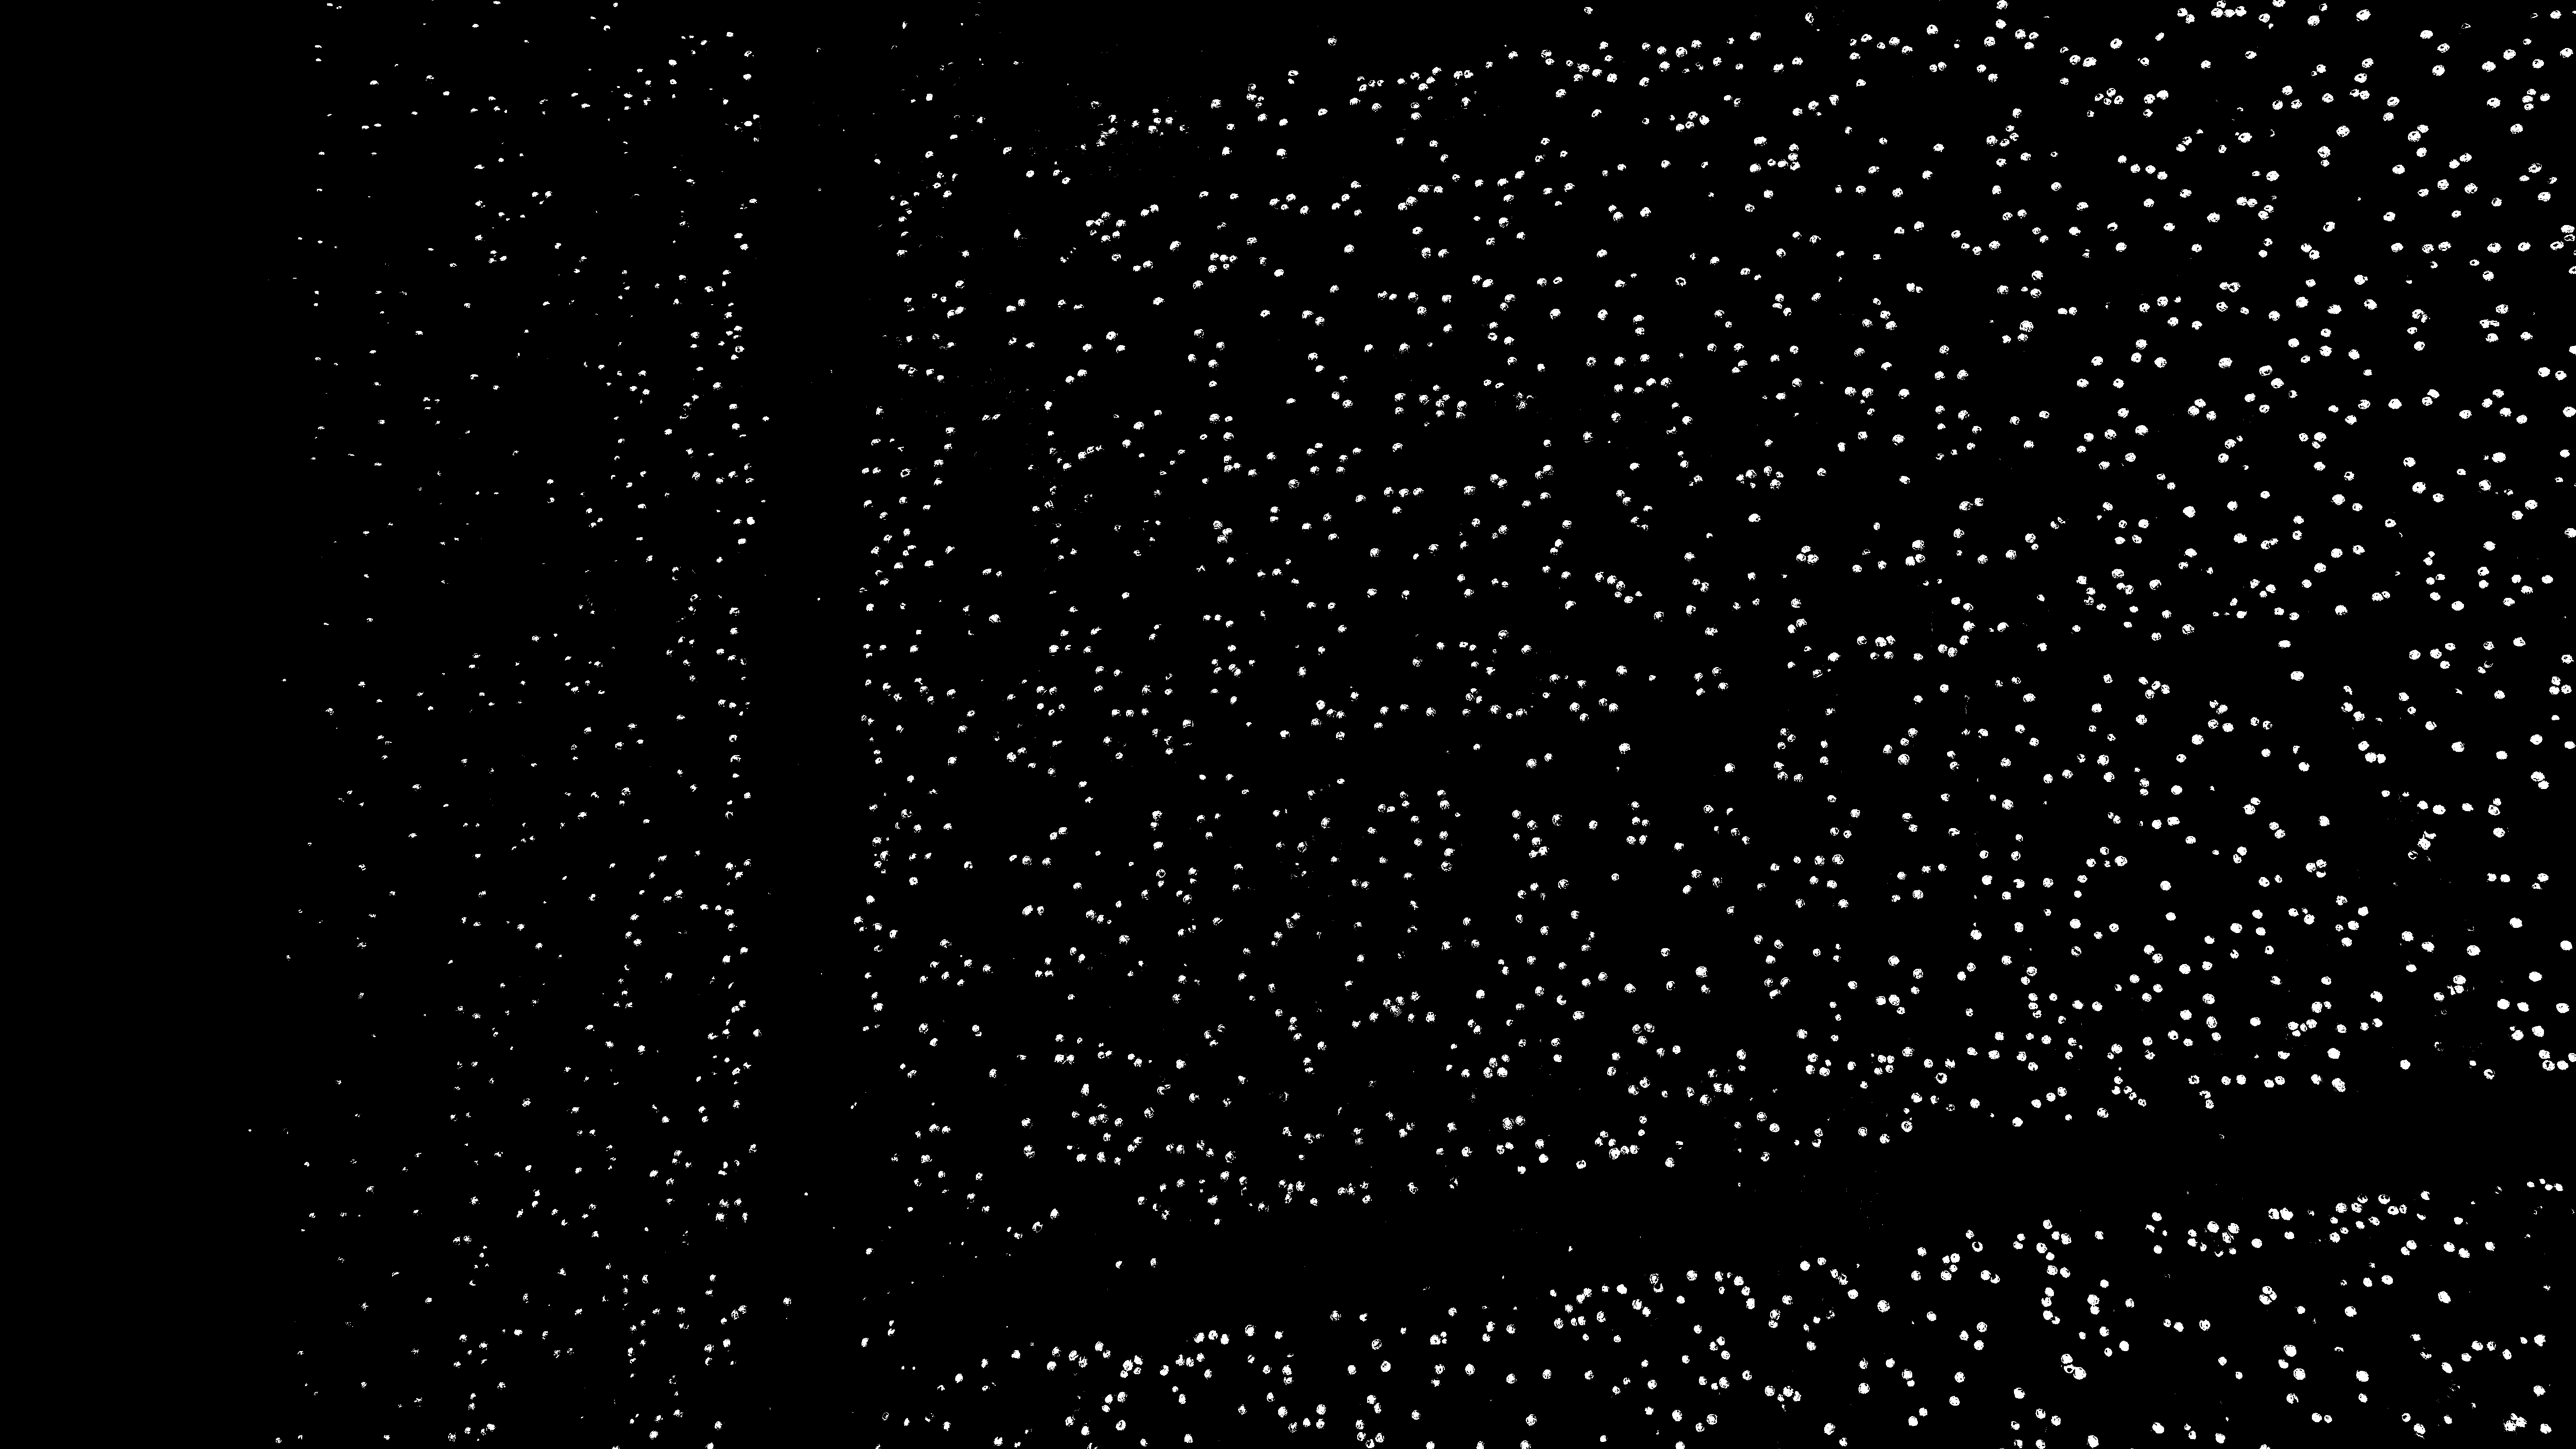
\includegraphics[width=0.8\textwidth]{../Figures/ex2_bgr_inrange.png}
\caption{Segmentation by range of BGR values}
\label{fig:bgrSeg}
\end{figure}

From visual inspection it can be seen that the RGB range segmentation segments the image quite well. 

\subsection{Segmentation by Range of CieLAB Color Values}
The same approach as segmentation by RGB color ranges is applied for the image converted to the CieLAB color space. By inspection of \ref{fig:histLab}, appropriate lower and upper boundaries of the color ranges are the mean value minus one standard deviation and the mean value plus two standard deviations. This will once again seperate the colors of the pumpkins from the color characteristics of the entire image. Part of the segmented image drawed back on the original image is seen in figure \ref{fig:labSeg}.

\begin{figure}[H]
\centering
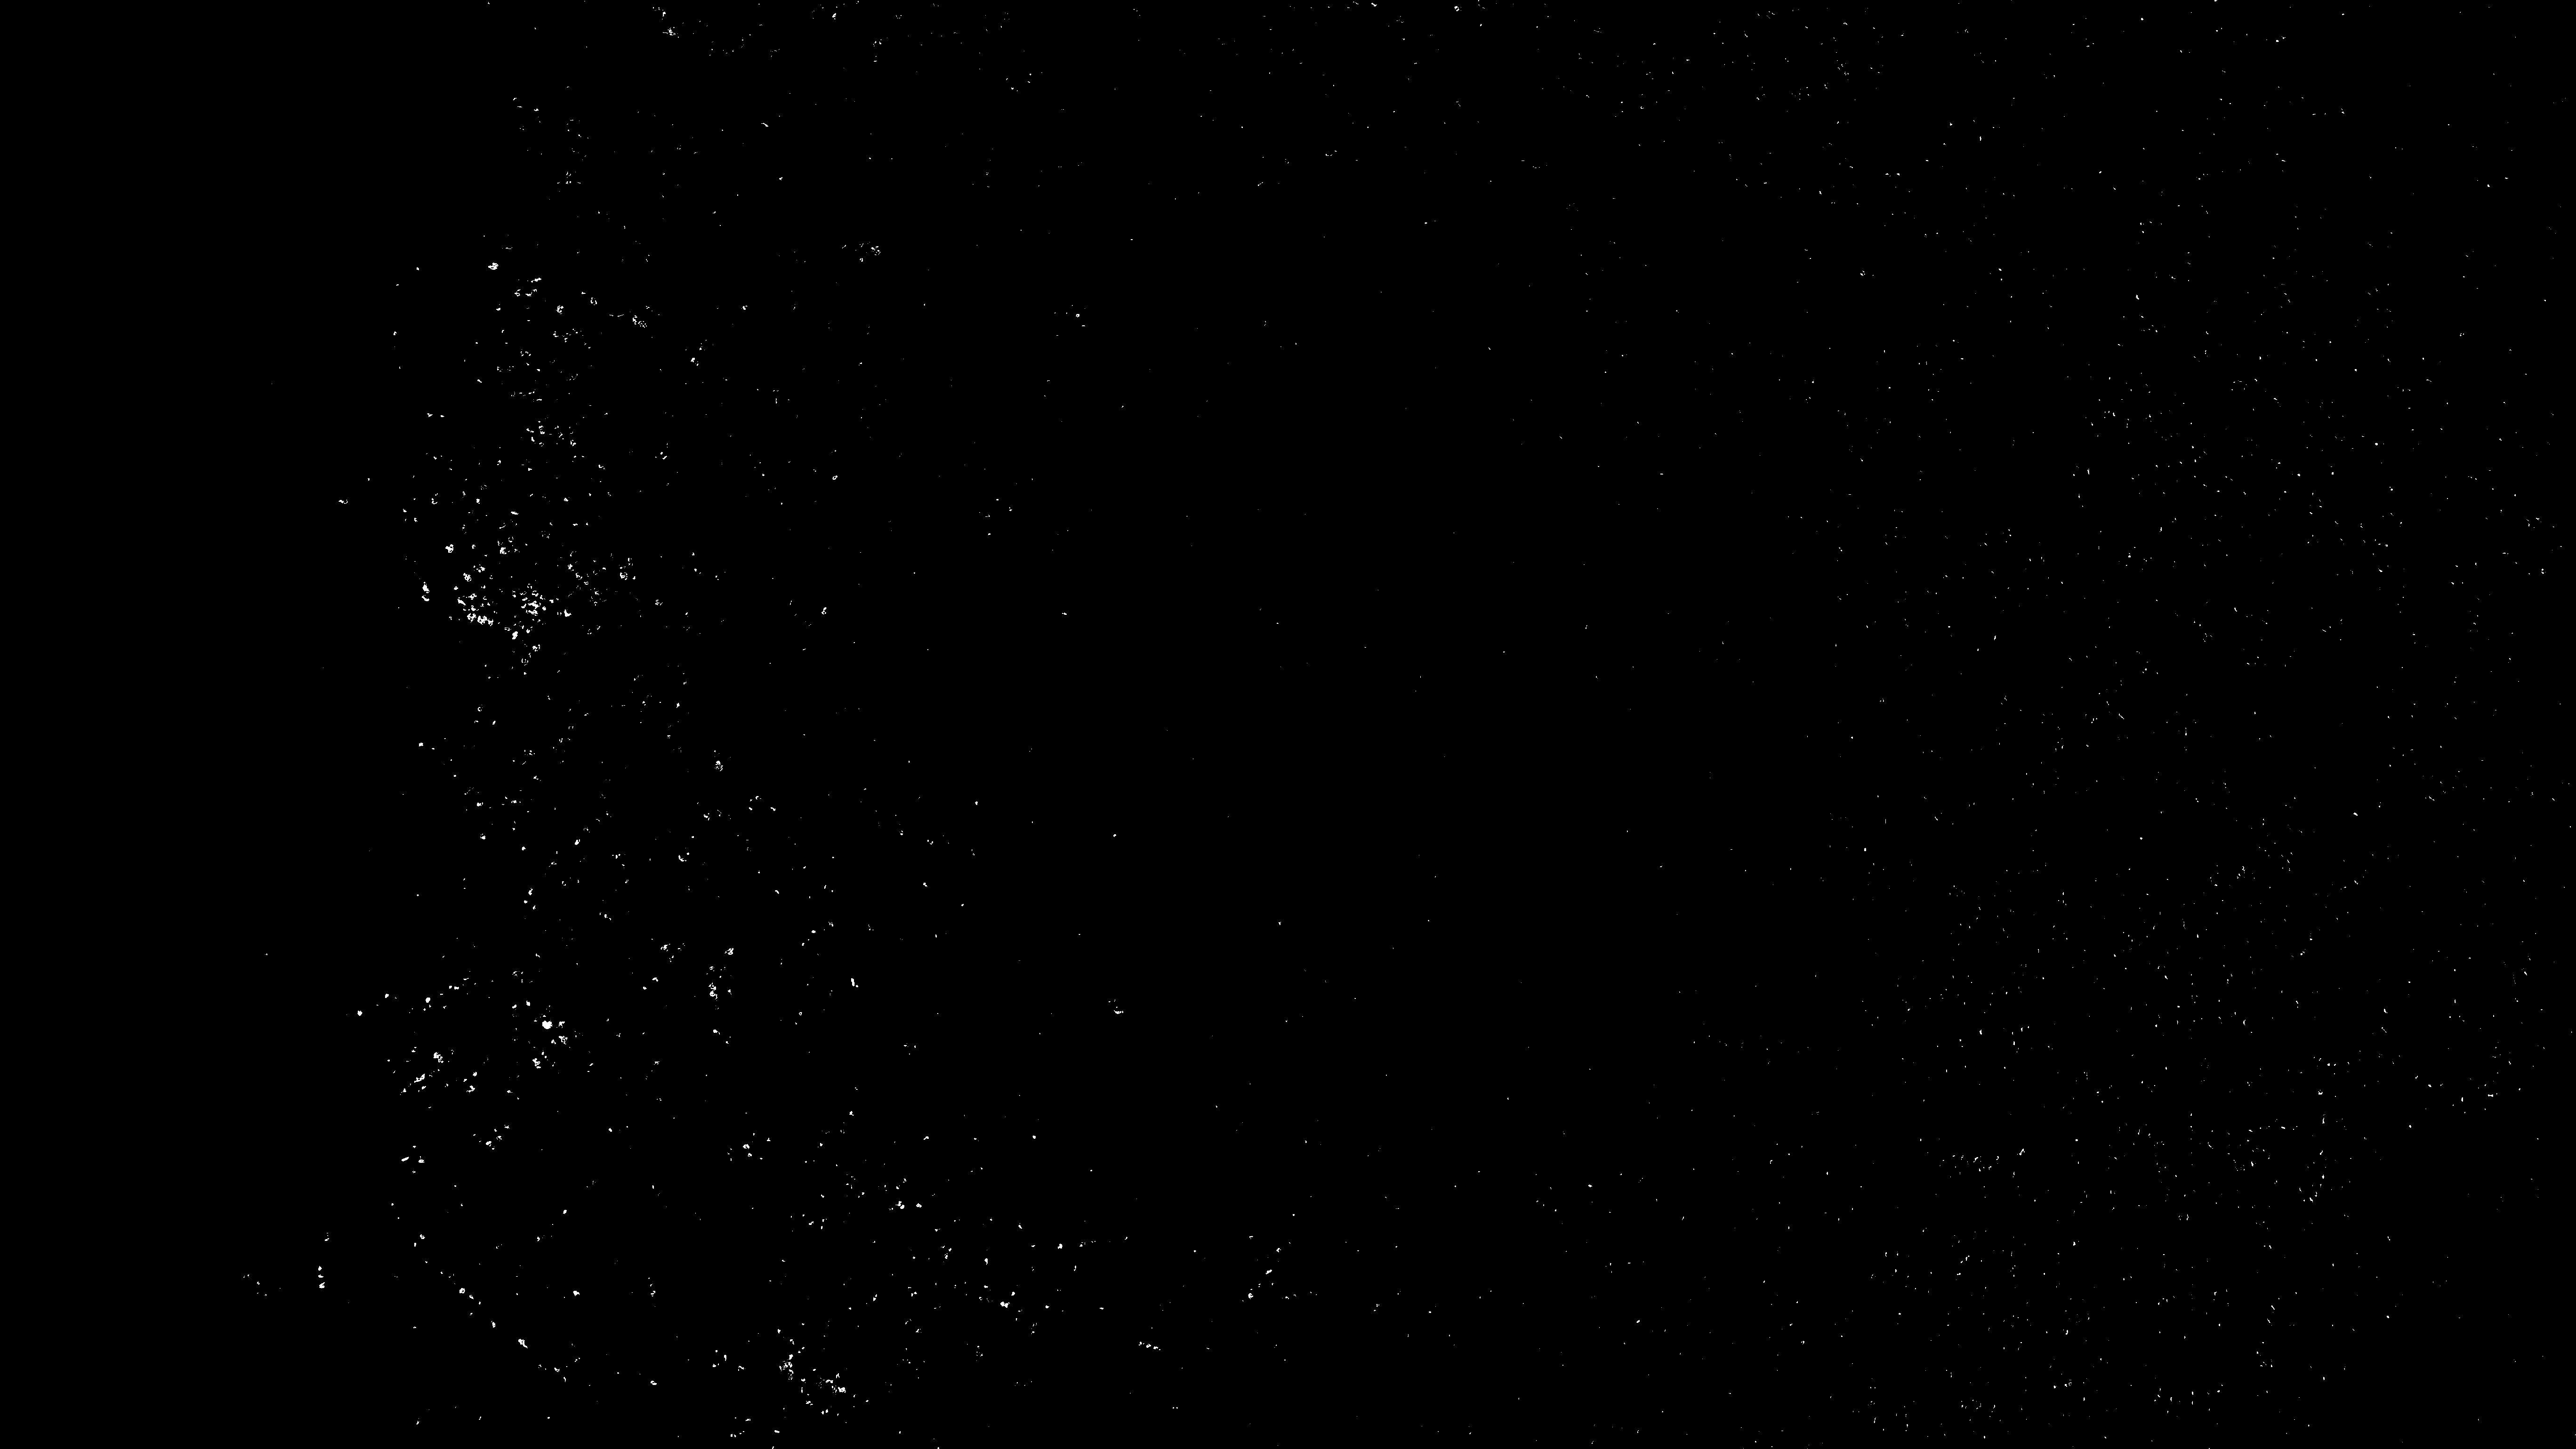
\includegraphics[width=0.8\textwidth]{../Figures/ex2_lab_inrange.png}
\caption{Segmentation by range of CieLAB values}
\label{fig:labSeg}
\end{figure}

It can be seen that the pumpkins are not as clearly seperated as with the BGR ranges. This is due to the fact that the standard deviations of the CieLAB channels are smaller than the BGR. A wider inclusion of the pumpkins could be obtained by widening the segmentation ranges, however this would result in a larger overlap of the segmentation ranges and the general distribution of color of the image in CieLAB space.

\subsection{Segmentation by Histogram Back Projection}
The histogram back projection was implemented based on the code example from OpenCV.\footnote{\url{https://docs.opencv.org/master/dc/df6/tutorial_py_histogram_backprojection.html}} The object of interest used was a pumpkin seperated to fit almost the entire image.\\
The results of the histogram back projection were of no use. A resulting image can be seen in figure \ref{fig:histSeg}.

\begin{figure}[H]
\centering
\includegraphics[width=0.8\textwidth]{../Figures/ex2_hist.png}
\caption{Segmentation by histogram back projection}
\label{fig:histSeg}
\end{figure}

It can be seen that the histogram backprojection doesn't remotely yield the expected results. This is most likely due to a error in the code. It was not corrected, and the results from this method were regarded useless.

\subsection{Segmentation by Distance from Mean in RGB Space}
The last applied method of segmentation was to segment the image by a maximum distance of each pixel from the RGB mean of a pumpkin. The approach was to make a distance image. The distance image would be in greyscale and each pixel would represent the normalized distance to the pumpkin RGB mean. In this way, the segmented image could easily be obtained by thresholding the distance image.

\subsubsection{Code for Generating Distance Image}
The code for generation of the distance image is explained here.\\
First, an image is created where each pixel represents the difference between the original pixel value and the mean value of a pumpkin as obtained in section \ref{sec:bombom} for each color channel. Here, the list \verb+bgr_val+ contains the said mean value:
\begin{verbatim}
img_sub = np.zeros(img_bgr.shape)
img_sub[:, :, 0] = np.subtract(img_bgr[:, :, 0], bgr_val[0])
img_sub[:, :, 1] = np.subtract(img_bgr[:, :, 1], bgr_val[1])
img_sub[:, :, 2] = np.subtract(img_bgr[:, :, 2], bgr_val[2])
\end{verbatim}
Then from the difference image a one channel image is created where each pixel is the Euclidean distance to the mean value:
\begin{verbatim}
img_dist = np.sqrt(np.multiply(img_sub[:, :, 0], img_sub[:, :, 0]) +
np.multiply(img_sub[:, :, 1], img_sub[:, :, 1]) + 
np.multiply(img_sub[:, :, 2], img_sub[:, :, 2]))
\end{verbatim}
Finally, all pixels are divided by the maximum Euclidean distance, yielding a normalized distance, the normalized distance is subtracted from 1 to make the pixel intensity decrease with increasing distance, and each pixel is multiplied by 255 and cast as integer to be in 8-bit format:
\begin{verbatim}
img_dist = np.divide(img_dist, img_dist.max())
img_dist = np.subtract(1, img_dist)
img_dist = np.multiply(img_dist, 255)
img_dist = img_dist.astype(int) 
\end{verbatim}
The reulting grey scale distance image can be seen in figure \ref{fig:bgrDist}.

\begin{figure}[H]
\centering
\includegraphics[width=0.8\textwidth]{../Figures/ex2_bgr_dist.png}
\caption{Segmentation by distance to pumpkin BGR mean}
\label{fig:bgrDist}
\end{figure}

It can be seen that the pumpkins in the brightly lit parts of the image are detected well by observing the white pixels. However, in the shadowy part of the image the pumpkins are not detected at all due to a large Euclidean distance from the overall pumpkin mean. Also the background is relatively light, meaning that the Euclidean distance between the background and the overall pumpkin mean is not sufficiently large.

\subsection{Final Words on Segmentation}
The best performing segmentation method was by far segmentation by range of BGR values. The method performed well in both the bright and the shady part of the image and only a negligible amount of pumpkins are not included in the segmentation. Furthermore, only a small amount of the background is included, which is also a success criteria for the segmentation method. This method is the one that will be used for the remainder of the project.\\
Finally, a filter is applied to the segmented image. The code for filtering the segmented image is contained in file \url{src/ex4.py}. The filter applied is a median blur filter.\\
By counting the pumpkins using the method described in section \ref{sec:countFast}, the resulting image was inspected and the efficiency of the filter was evaluated by the number of non pumpkins marked as pumpkins. An appropriate filter size was chosen to be 5.

\end{document}